\documentclass[12pt]{article}

\usepackage{macros}

\title{Lecture 2 for EE127 (Fall 2018): Vectors and Functions}
\author{Scribes: Yagna Patel}
\date{8/28/2018}
\begin{document}


\maketitle

\section{Vectors}
We are mostly familiar with values represented by a single number. For example, $3$ seconds, $60$ mi/h, etc. These are all \textbf{scalar} values. One thing scalar values lack is direction. Vectors are able to encode both size and direction. For example, velocity is a vector quantity since it tells us the direction an object is traveling along with its speed, while speed is a scalar quantity.

\noindent We usually write a vector in column format: $$\mathbf{x} = \begin{bmatrix}x_1 \\ x_2 \\ \vdots \\ x_n\end{bmatrix}$$ Here, each element $x_i$, is the $i$-th component of the vector. There are a total of $n$ components in $\mathbf{x}$. The total number of components is the \textbf{dimension} of the vector. $\mathbf{x}$ is an $n$-dimensional vector. Now, when each of the components is a real number, i.e. $x_i\in\mathbb{R}$, we call $\mathbf{x}$ a real vector, and we write $\mathbf{x}\in\mathbb{R}^n$. If for some vector $\mathbf{y}$, $y_i\in\mathbb{C}$, then $\mathbf{y}\in\mathbb{C}^n$.

\noindent Now, one useful function on vectors is the \textbf{transpose}. The transpose transforms a column vector into a row vector, and vice versa. For example, the transpose of $\mathbf{x}$, is written as $$\mathbf{x}^\top = \begin{bmatrix}x_1 & x_2 & \cdots  & x_n\end{bmatrix}$$ The transpose also has a few useful properties:
\begin{itemize}
\item Let $\mathbf{x},\mathbf{y}\in\mathbb{R}^n$. Then, $$(\mathbf{x}+\mathbf{y})^\top = \mathbf{x}^\top + \mathbf{y}^\top$$
\item Let $\mathbf{x},\mathbf{y}\in\mathbb{R}^n$. Then, $$(\mathbf{x}\mathbf{y})^\top = \mathbf{y}^\top\mathbf{x}^\top$$
\item Let $\mathbf{x}\in\mathbb{R}^n$. Then, $$\left(\mathbf{x}^\top\right)^\top = \mathbf{x}$$
\end{itemize} 

\section{Vector Spaces}
\begin{definition}
Let $\mathbb{F}$ be a field (e.g. $\mathbb{R}$). A \textbf{vector space}, $V$, is a collection of vectors with two operations:
\begin{itemize}
\item The first operation is vector addition. Let $\mathbf{x},\mathbf{y}\in V$. Vector addition takes $\mathbf{x}$ and $\mathbf{y}$ and produces $$\mathbf{x}+\mathbf{y} = \begin{bmatrix}x_1 \\ x_2 \\ \vdots \\ x_n\end{bmatrix}+\begin{bmatrix}y_1 \\ y_2 \\ \vdots \\ y_n\end{bmatrix} = \begin{bmatrix} x_1 + y_1 \\ x_2+y_2 \\ \vdots \\ x_n + y_n\end{bmatrix}\in V$$. 
\item The second operation is scalar multiplication. Let $c\in\mathbb{F}$, where $\mathbb{F}$, and $\mathbf{x}\in V$. Scalar multiplication takes $c$ and $\mathbf{x}$ and produces $$c\mathbf{x} = c\begin{bmatrix}x_1 \\ x_2 \\ \vdots \\ x_n\end{bmatrix} = \begin{bmatrix}cx_1 \\ cx_2 \\ \vdots \\ cx_n\end{bmatrix}\in V$$
\end{itemize}
such that the following axioms are satisfied:
\begin{itemize}
\item \textit{Existence of identity.} There exists a vector $\mathbf{0}\in V$ such that for every $\mathbf{v}\in V$, $\mathbf{0}+\mathbf{v} = \mathbf{v}$. Furthermore, there exists a vector $1\in \mathbb{F}$ such that for every $\mathbf{v}\in V$, $1\mathbf{v} = \mathbf{v}$.
\item \textit{Existence of inverses.} For every $\mathbf{v}\in V$, there exists a vector $-\mathbf{v}\in V$ such that $\mathbf{v} + (-\mathbf{v}) = 0$. 
\item \textit{Associativity.} For every $\mathbf{x},\mathbf{y},\mathbf{z}\in V$, $$(\mathbf{x} + \mathbf{y}) + \mathbf{z} = \mathbf{x} + (\mathbf{y} + \mathbf{z})$$ Furthermore, for any $c,d\in\mathbb{F}$ and $\mathbf{x}\in V$, $$(cd)\mathbf{x} = c(d\mathbf{x})$$
\item \textit{Distributivity.} For any $c,d\in\mathbb{F}$ and $\mathbf{x},\mathbf{y}\in V$, $$(c + d)\mathbf{x} = c\mathbf{x} + d\mathbf{x}\quad\text{and}\quad c(\mathbf{x} + \mathbf{y}) = c\mathbf{x} + c\mathbf{y}$$

\end{itemize}
\end{definition}
\noindent Notice that the resulting vectors from both operations must lie in the vector space. This property is called \textbf{closure} property. Vector spaces must satisfy this closure property. 
\begin{example} $\mathbb{R}^n$ is a vector space over $\mathbb{R}$ under vector addition and scalar multiplication.\end{example}
\begin{example} The set of polynomials with real coefficients and with degree $\leqslant n$, i.e. $P_n = \left\{\sum_{i=0}^n c_ix^i \mid c_i\in\mathbb{R}\right\}$ is a vector space under polynomial addition and polynomial multiplication.\end{example}

\section{Subspaces and Span}
\begin{definition}
Let $\mathbf{F}$ be a field. A subspace of a vector space $V$ is a nonempty subset $W\subseteq V$ such that
\begin{itemize}
\item $\mathbf{0}\in W$.
\item For every $\mathbf{x},\mathbf{y}\in W$, $\mathbf{x}+\mathbf{y}\in W$.
\item For every $\mathbf{x}\in W$ and $c\in\mathbb{F}$, $c\mathbf{x}\in W$.
\end{itemize}
\end{definition}
\begin{example}
The set of solutions $(x,y)\in\mathbb{R}^2$ of $ax + by=0$ where $a,b\in\mathbb{R}$ forms a plane in $\mathbb{R}^2$. This plane passes through the origin and it forms a vector space which is a subspace of $\mathbb{R}^2$. Notice that if this plane did not pass through the origin, then it would no longer be a vector space since it does not satisfy the axiom of the existence of the identity element.
\end{example}
\noindent We can also add two subspaces together, known as taking the direct sum of subspaces. Let $V,W$ be two subspaces. The direct sum of $V$ and $W$, denoted as $V \oplus W$, is the set of vectors of the form $\mathbf{x} + \mathbf{y}$, where $\mathbf{x}\in V$ and $\mathbf{y}\in W$. Furthermore, $V \oplus W$ is also a subspace. 
\begin{definition}
Let $\mathbb{F}$ be a field. A \textbf{linear combination} of a set of vectors $S$ in a vector space $V$, is the finite sum of the scalar multiples of the vectors in $S$. If $c_i\in\mathbb{F}$ and $\mathbf{x}_i\in V$, then $$c_1\mathbf{x}_1 + \ldots + c_n\mathbf{x}_n$$ is a linear combination.
\end{definition}
\begin{example}
$\begin{bmatrix}-2 \\ -1 \\ 0\end{bmatrix}$ is a linear combination of $\begin{bmatrix}1 \\ 2 \\ 3\end{bmatrix}$ and $\begin{bmatrix}4 \\ 5 \\ 6\end{bmatrix}$ since $$\begin{bmatrix}-2 \\ -1 \\ 0\end{bmatrix} = 2\begin{bmatrix}1 \\ 2 \\ 3\end{bmatrix} + (-1)\begin{bmatrix}4 \\ 5 \\ 6\end{bmatrix}$$
\end{example}
\begin{definition}
The set of all linear combinations of vectors in $S\subseteq V$ is the \textbf{span} of $S$.
\end{definition}
\noindent Notice that $\operatorname{span}(S)$ forms a subspace. 

\section{Bases and Dimensions}
\begin{definition}
Let $\mathbb{F}$ be a field. A subset of vectors $S\subseteq V$ is linearly independent if no vector in $S$ can be expressed as a linear combination of the others, i.e. $$c_1\mathbf{x}_1 + \ldots + c_n\mathbf{x}_n = 0$$ with $c_i\in\mathbb{F}$ and $\mathbf{x}_i\in S$ implies $c_1=c_2=\cdots = c_n=0$.
\end{definition}
\noindent A \textbf{basis} of a vector space is the set of all vectors that can be used as coordinates for that space. A basis must be a set that spans the vector space and is linearly independent. 
\noindent If $B$ is the basis of some vector space $V$, then the dimension of $V$ is the number of elements in $B$, i.e. $\dim(V) = |B|$.
\begin{example}
One basis for $\mathbb{R}^3$ is $$\{(1,0,0),(0,1,0),(0,0,1)\}$$ We can write any element in $\mathbb{R}^3$ using these three elements. Additionally, $\dim(\mathbb{R}^3) = 3$.
\end{example}
\noindent Now, if we have a basis $B$ for a subspace $S$, then we can write any element in $S$ as a linear combination of the elements in $B$, i.e. for any $\mathbf{x}\in S$, $$\mathbf{x}=\sum_{i=1}^{|B|} c_i\mathbf{x}_i$$ where $c_i\in\mathbb{F}$ where $\mathbb{F}$ is some field.

\section{Affine Spaces}
Recall in Example 3.2 we had noted that if a plane did not pass through the origin, then it would no longer be a vector space. The plane did resemble a vector space in many ways. However, instead of a vector space, this is an affine space. 
\begin{definition}
A set $S$ is affine if $\mathbf{x},\mathbf{y}\in S$ implies that $(1-\lambda)\mathbf{x} + \lambda\mathbf{y}\in S$ for every $\lambda\in \mathbb{F}$ for some field $\mathbb{F}$.
\end{definition}
\noindent If we think about this geometrically, this definition is saying that a set is affine if whenever two points are in a set, the line crossing through these points must also be in the set. 

\noindent Now, to understand what an affine space is, it's best to first look at the difference between a vector space and an affine space. Recall that a vector space is closed under any linear combination of its vectors, i.e. if $\mathbb{F}$ is some field, $V$ is a vector space, $\mathbf{x},\mathbf{y}\in V$, and $c, d\in\mathbb{F}$, then $c\mathbf{x} + d\mathbf{y}\in V$. Now, an affine space is closed under affine combinations of its vectors, i.e. if $\mathbb{F}$ is some field, $A$ is an affine space, $\mathbf{x},\mathbf{y}\in A$, and $\lambda\in \mathbb{F}$, then $(1-\lambda)\mathbf{x} + \lambda\mathbf{y}\in A$.

\begin{definition}
If $V$ is a vector space, and $W$ is a subspace of $V$, then for $\mathbf{x}\in V\setminus W$, $$\mathbf{x} + W = \{\mathbf{x} + \mathbf{y}\,:\,\mathbf{y}\in W\}$$ is an affine subspace of $V$.
\end{definition}
\noindent Simply put, if you take any vector space and shift it away from the origin, the result is an affine subspace. Notice that the equation of the line in Definition 5.1 looks familiar to the definition of convex sets. In fact, the notion of affine sets is related to convex sets. An affine set contains the line crossing through any two points in the set, while a convex set contains the line segment between any two points in the set. Notice the distinction between a "line segment" and a "line crossing through". Therefore, all affine sets are also convex. However, not all convex sets are affine.

\section{Norms and $\ell_p$ norms}
Similar to a metric, a norm on a vector space $V$ is a real-valued function which maps any vector $\mathbf{x}\in V$ into a real number $\|\mathbf{x}\|$. 
\begin{definition}
A function from a vector space $V\to \mathbb{R}$ is a norm if the following properties hold:
\begin{itemize}
\item For every $\mathbf{x}\in V$, $\|x\|\geqslant 0$ and $\|\mathbf{x}\|=0$ if and only if $\mathbf{x} = 0$.
\item For any $\mathbf{x},\mathbf{y}\in V$, $\|\mathbf{x}+\mathbf{y}\|\leqslant \|\mathbf{x}\|+\|\mathbf{y}\|$. \item For any scalar $c$ and $\mathbf{x}\in V$, $\|c\mathbf{x}\| = |c|\|\mathbf{x}\|$. \end{itemize}
\end{definition}
\noindent The first bullet is essentially requiring $\mathbf{0}$ have zero length, and every non-zero vector have positive length. The second bullet is the triangle inequality: it's always faster to go to a place directly rather than taking a detour. The third bullet is saying that multiplying a vector by some scalar scales the length of the vector by a factor of the scalar value.

\begin{definition}
The $\ell_p$ norm is defined as $$\|\mathbf{x}|\|_p = \left(\sum_{k=1}^n |x_k|^p\right)^{1/p},\quad 1\leqslant p<\infty$$
\end{definition}
\noindent Now, we will look at some cases of the $\ell_p$ norm:
\begin{enumerate}
\item $\ell_0$ norm. Let's work out $\|\mathbf{x}\|_0$: $$\|\mathbf{x}\|_0 = \left(\sum_{k=1}^n |x_k|^0\right)^{1/0}$$ Now, clearly there's something wrong here. Although, it doesn't make sense to have an $\ell_0$ norm, there does exist one! The $\ell_0$ norm is the cardinality function defined as the number of non-zero elements of a vector, i.e. $$\|\mathbf{x}\|_0 =  |\{i\,:\, x_i \neq 0\}|$$
\begin{example}
If $\mathbf{x} = \begin{bmatrix}1 \\ -1 \\ 0\end{bmatrix}$, then $\|x\|_0 = 2$.
\end{example}
\item $\ell_1$ norm. Let's work out $\|\mathbf{x}\|_1$: $$\|\mathbf{x}\|_1 = \left(\sum_{k=1}^n |x_k|^1\right)^{1/1} = \sum_{k=1}^n |x_k|$$
This norm is simply the sum of the absolute values of all the elements of vector $\mathbf{x}$. 
\begin{example}
If $\mathbf{x} = \begin{bmatrix}1 \\ -1 \\ 0\end{bmatrix}$, then $\|x\|_1 = |1| + |-1| + |0| = 2$.
\end{example}
\item $\ell_2$ norm. Let's work out $\|\mathbf{x}\|_2$: $$\|\mathbf{x}\|_2 = \left(\sum_{k=1}^n |x_k|^2\right)^{1/2} = \sqrt{\sum_{k=1}^n x_k^2}$$
This norm is commonly referred to as the euclidean norm. 
\begin{example}
If $\mathbf{x} = \begin{bmatrix}1 \\ -1 \\ 0\end{bmatrix}$, then $\|x\|_2 = \sqrt{(1)^2 + (-1)^2 + (0)^2} = \sqrt{2}$.
\end{example}

\item $\ell_\infty$ norm. This is another special norm. The infinity norm of a vector $\mathbf{x}$ is defined as the maximum of the absolute values of each of its elements, i.e. $$\|\mathbf{x}\|_\infty = \max_i |x_i|$$
\begin{example}
If $\mathbf{x} = \begin{bmatrix}1 \\ -1 \\ 0\end{bmatrix}$, then $\|x\|_\infty = \max\{|1|,|-1|,|0|\} = 1$.
\end{example}
\end{enumerate}


\section{Inner Products}
\begin{definition}
Let $\mathbf{x}, \mathbf{y}\in\mathbb{R}^n$. The dot product of $\mathbf{x}$ and $\mathbf{y}$, denoted by $\mathbf{x}\cdot \mathbf{y}$ is defined as $$\mathbf{x}\cdot\mathbf{y} = \mathbf{x}^\top\mathbf{y} =\sum_{k=1}^n x_ky_k = x_1y_1 + \ldots + x_ny_n$$
\end{definition}
\noindent The dot product is a special case of an inner product in euclidean space. Inner products are a generalized version of the dot product. 
\begin{definition}
The inner product on a vector space $V$ is a function that takes every ordered pair $(x,y)$ of the elements of $V$ and maps it to a number $\langle x,y\rangle\in \mathbb{F}$, where $\mathbb{F}$ is some field, and has the following properties:
\begin{itemize}
\item For every $\mathbf{x}\in V$, $\langle \mathbf{x}, \mathbf{x}\rangle \geqslant 0$ and  $\langle \mathbf{x}, \mathbf{x}\rangle = 0$ if and only if $\mathbf{x} = 0$.
\item For every $\mathbf{x},\mathbf{y},\mathbf{z}\in V$, $\langle \mathbf{x} + \mathbf{y}, \mathbf{z}\rangle = \langle \mathbf{x}, \mathbf{z}\rangle + \langle \mathbf{y}, \mathbf{z}\rangle$.
\item For every $\lambda\in\mathbb{F}$ and $\mathbf{x},\mathbf{y}\in V$, $\langle\lambda\mathbf{x},\mathbf{y}\rangle = \lambda\langle\mathbf{x},\mathbf{y}\rangle$.
\item For every $\mathbf{x},\mathbf{y}\in V$, $\langle\mathbf{x},\mathbf{y}\rangle = \langle\mathbf{y},\mathbf{x}\rangle$.
\end{itemize}
\end{definition}
\noindent If a vector space has the above inner product structure, it is referred to as an \textbf{inner product space}. Additionally, the inner product induces a norm: $$\|\mathbf{x}\| = \sqrt{\langle \mathbf{x}, \mathbf{x}\rangle}$$

\noindent Now, the definition of the dot product we saw earlier can be given a geometric interpretation in terms of the angle created between the two vectors. 
\begin{definition}
Let $\mathbf{x}, \mathbf{y}\in\mathbb{R}^n$ and let $\theta$ be the angle between the two vectors. The dot product of $\mathbf{x}$ and $\mathbf{y}$ is $$\mathbf{x}\cdot \mathbf{y} = \|\mathbf{x}\|\|\mathbf{y}\|\cos\theta$$
\end{definition}
\noindent Therefore, to get the angle between two vectors, we can solve for $\cos\theta$: $$\cos\theta = \frac{\|\mathbf{x}\|\|\mathbf{y}\|}{\mathbf{x}\cdot \mathbf{y}}$$
\pagebreak
\begin{figure}[h!]\begin{center}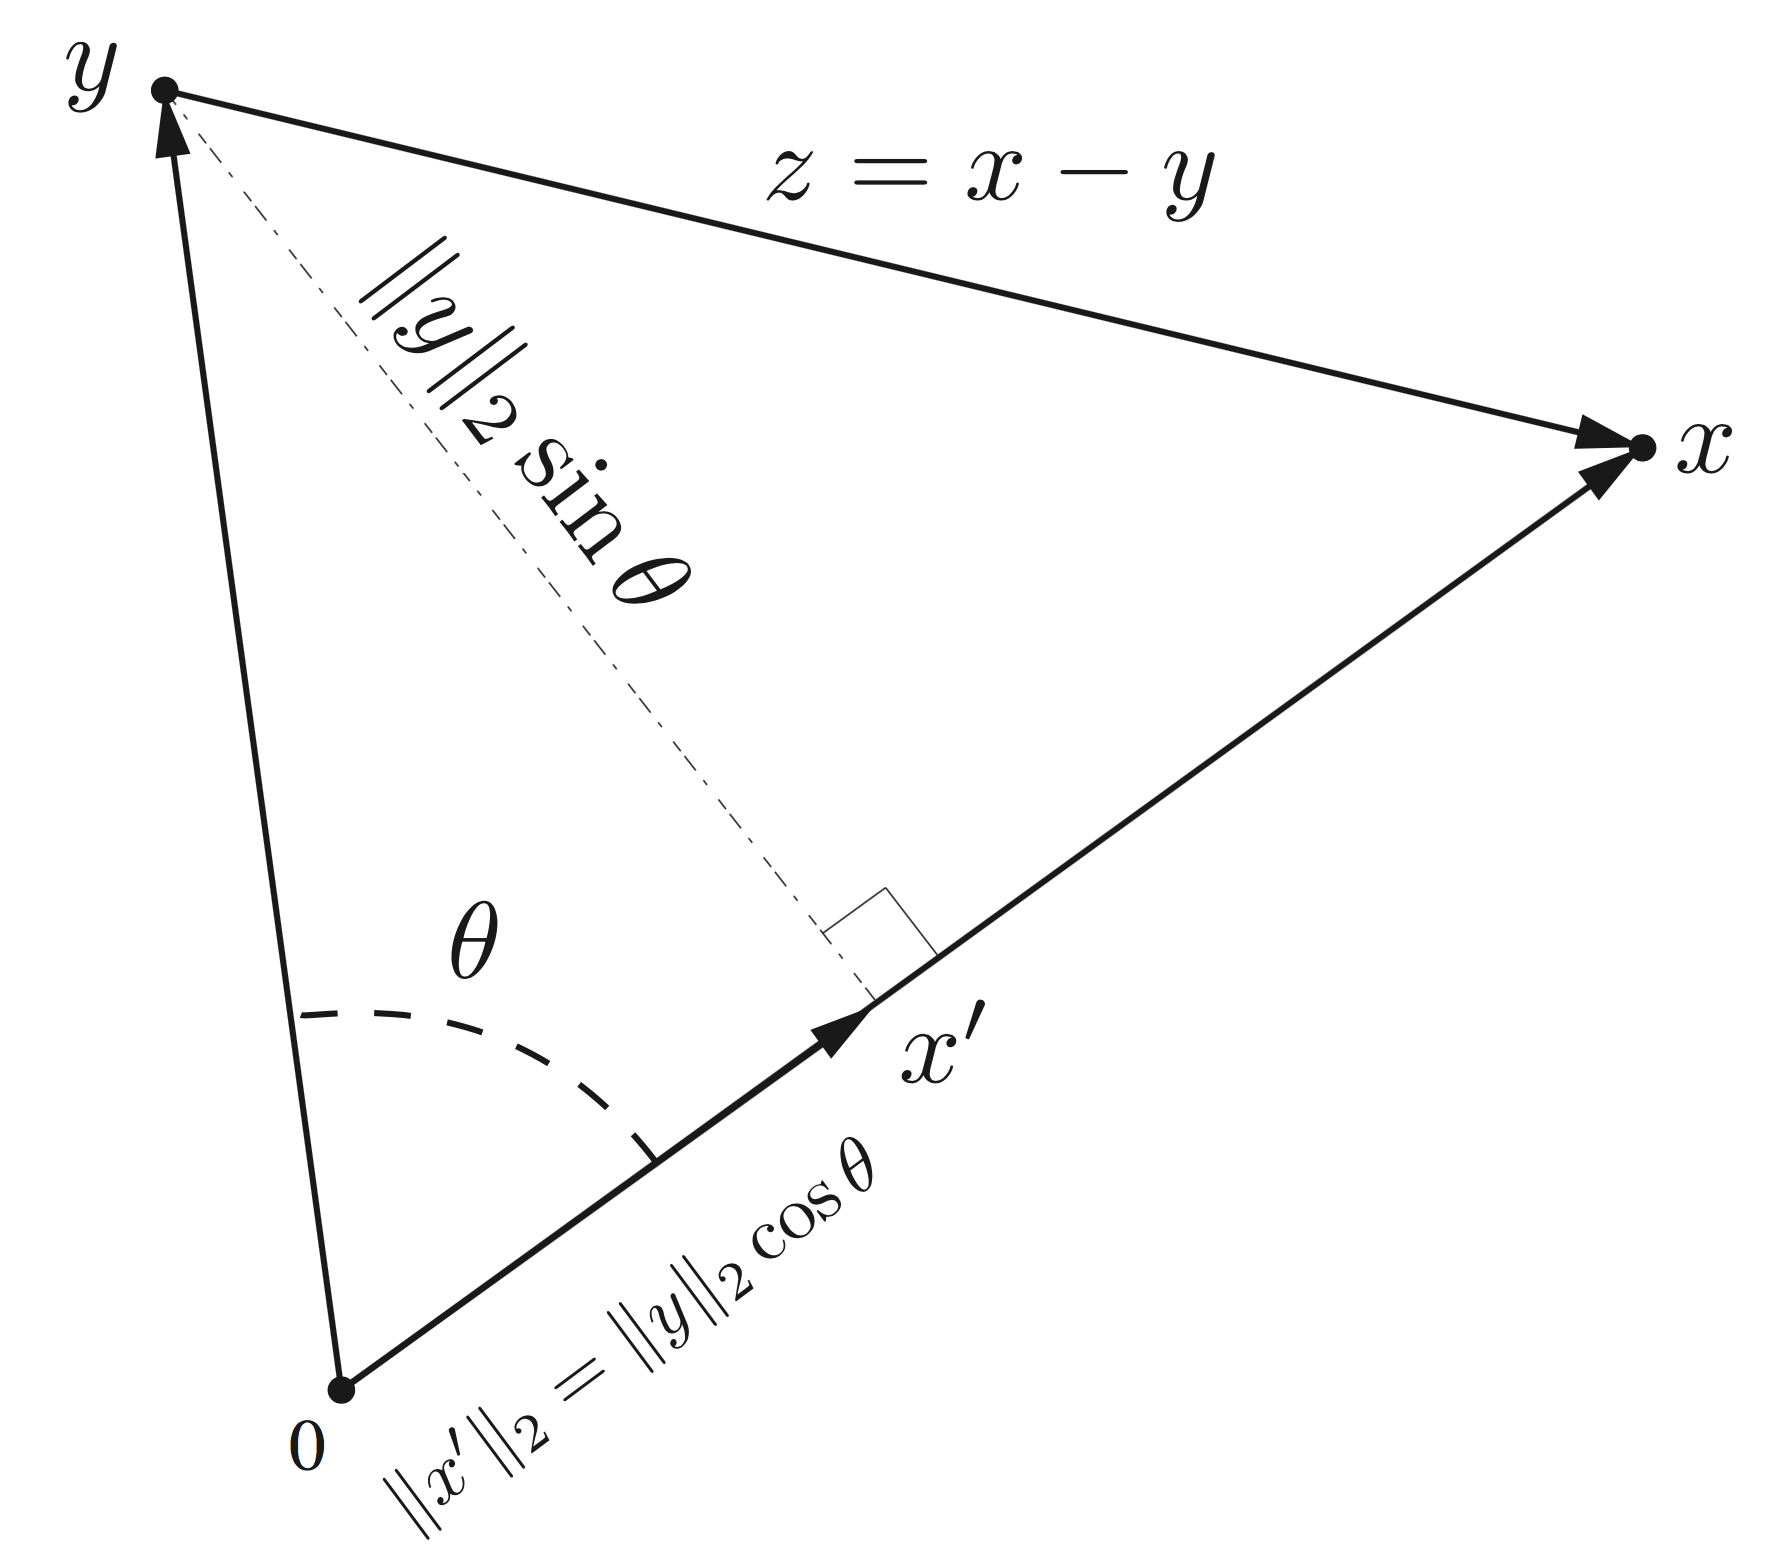
\includegraphics[scale=0.2]{figures/angles}\caption{Angle Between Two Vectors}\end{center}\end{figure}

\noindent In Figure 1 we see the relation between the length and the angle. Notice that when $\theta = \pm 90^\circ$, i.e. $\mathbf{x}\perp\mathbf{y}$, we find that $\mathbf{x}\cdot \mathbf{y} = 0$. When the angle between two vectors is $\pm 90^\circ$, the vectors are \textbf{orthogonal}. Now, notice that when $\theta = 0^\circ, 180^\circ$, we have that $\mathbf{x}\cdot \mathbf{y} = 1$. If we visualize this, the two vectors are parallel to each other. 

\begin{definition}
Two vectors $\mathbf{x},\mathbf{y}\in \mathcal{X}$, where $\mathcal{X}$ is an inner product space, are \textbf{orthogonal} if $\langle \mathbf{x}, \mathbf{y}\rangle = 0$. Orthogonality of two vectors $\mathbf{x},\mathbf{y}\in \mathcal{X}$ is symbolized by $\mathbf{x}\perp\mathbf{y}$. 
\end{definition}

\begin{definition}
Non-zero vectors $\mathbf{x}_1,\ldots,\mathbf{x}_d\in\mathcal{X}$, where $\mathcal{X}$ is an inner product space, are said to be \textbf{mutually orthogonal} if $\langle \mathbf{x}_i, \mathbf{x}_j\rangle = 0$ whenever $i\neq j$. 
\end{definition}
\noindent Essentially, this definition is saying that non-zero vectors are mutually orthogonal if they are orthogonal to all other vectors in the collection of vectors.
\begin{definition}
If $U$ is a subset of $V$, where $V$ is an inner product space, then the orthogonal complement of $U$, denoted by $U^\perp$, is the set of all vectors in $V$ that are orthogonal to every vector in $U$, i.e. $$U^\perp = \{\mathbf{x}\in V\,:\, \langle \mathbf{x},\mathbf{y}\rangle = 0,\,\forall \mathbf{y}\in U\}$$
\end{definition}

\noindent For example, suppose that $U$ is a line in $\mathbb{R}^3$ such that it passes through the origin. $U^\perp$ would be the plane containing the origin that is perpendicular to $U$. On the other hand, if $U$ is now a plane in $\mathbb{R}^3$ such that it passes through the origin. $U^\perp$ would be the line containing the origin that is perpendicular to $U$.

\noindent Some properties of orthogonal complements are:
\begin{itemize}
\item If $U\subset V$, then $U^\perp$ is a subspace of $V$.
\item $\{0\}^\perp = V$.
\item If $U$ is a subset of $V$, then $U\cap U^\perp\subset \{0\}$.
\end{itemize}
\begin{theorem}
Suppose that $U$ is a finite-dimensional subspace of $V$. Then $$V = U\oplus U^\perp$$
\begin{proof}
Suppose that $\mathbf{x}\in V$. Let $\mathbf{e}_1, \ldots, \mathbf{e}_m$ be an orthonormal basis of $U$. Let $$\mathbf{y}=\langle \mathbf{x}, \mathbf{e}_1 \rangle \mathbf{e}_1 +\ldots  + \langle \mathbf{x}, \mathbf{e}_m \rangle \mathbf{e}_m$$ Then, $$\langle \mathbf{x}-\mathbf{y}, \mathbf{e}_k\rangle = \langle \mathbf{x}, \mathbf{e}_k\rangle - \langle \mathbf{y}, \mathbf{e}_k\rangle = 0\quad\text{for }j=1,\ldots,m$$
The above step uses the additive property of inner products. Therefore, $\mathbf{x}-\mathbf{y}\in U^\perp$. Now, notice that $$\mathbf{x} = \mathbf{y} + (\mathbf{x}-\mathbf{y})$$Therefore, $\mathbf{x}\in U+U^\perp$. Hence, $V=U+U^\perp$.
\end{proof}
\end{theorem}
\begin{corollary}
Suppose that $U$ is a finite-dimensional subspace of $V$. Then, $$\dim U^\perp = \dim V - \dim U$$
\end{corollary}
\begin{definition}
A collection of vectors $S = \{\mathbf{x}_1,\ldots,\mathbf{x}_d\}$ is said to be orthonormal if, for $i,j=1,\ldots,d$, $$\langle \mathbf{x}_i,\mathbf{x}_j\rangle = \begin{cases}0 & \text{if } i\neq j\\ 1 & \text{if }i=j\end{cases}$$
\end{definition}

\noindent Essentially, $S$ is orthonormal if every element has unit norm, and all elements are orthogonal to each other. A collection of orthonormal vectors $S$ forms an orthonormal basis for the span of $S$.

\noindent Now, in the dot product, since $|\cos\theta|\leqslant 1$, we can deduce the following from the dot product:
$$|\mathbf{x}\cdot \mathbf{y}|\leqslant \|\mathbf{x}\|_2\|\mathbf{y}\|_2$$
This result is famously known as the \textbf{Cauchy-Schwartz inequality}. Holder's inequality is a generalization of the Cauchy-Schwartz inequality:
\begin{theorem}
Let $p,q>1$ such that $\frac{1}{p} + \frac{1}{q} = 1$ and let $a_k, b_k$ be sequences of real numbers. Holder's inequality states that $$\sum_{k=1}^n |a_kb_k|\leqslant \left(\sum_{k=1}^n|a_k|^p\right)^{1/p}\left(\sum_{k=1}^n|b_k|^q\right)^{1/q}$$
\end{theorem}
\noindent Notice that with our knowledge of $\ell_p$ norms, Holder's inequality becomes:
$$|\mathbf{a}\cdot \mathbf{b}|\leqslant \|\mathbf{a}\|_p\|\mathbf{b}\|_q$$

\section{Maximization of Inner Products over Norm Balls}
\begin{definition}
A norm ball is defined as the set of $$B_p(r) = \left\{\mathbf{x}\in\mathbb{R}^n\,:\,\sum_{k=1}^n |x_k|^p\leqslant r^p\right\}$$
\end{definition}
\noindent Here, you can think of $r$ as the radius of the ball.

 \begin{figure}[h!]\begin{center}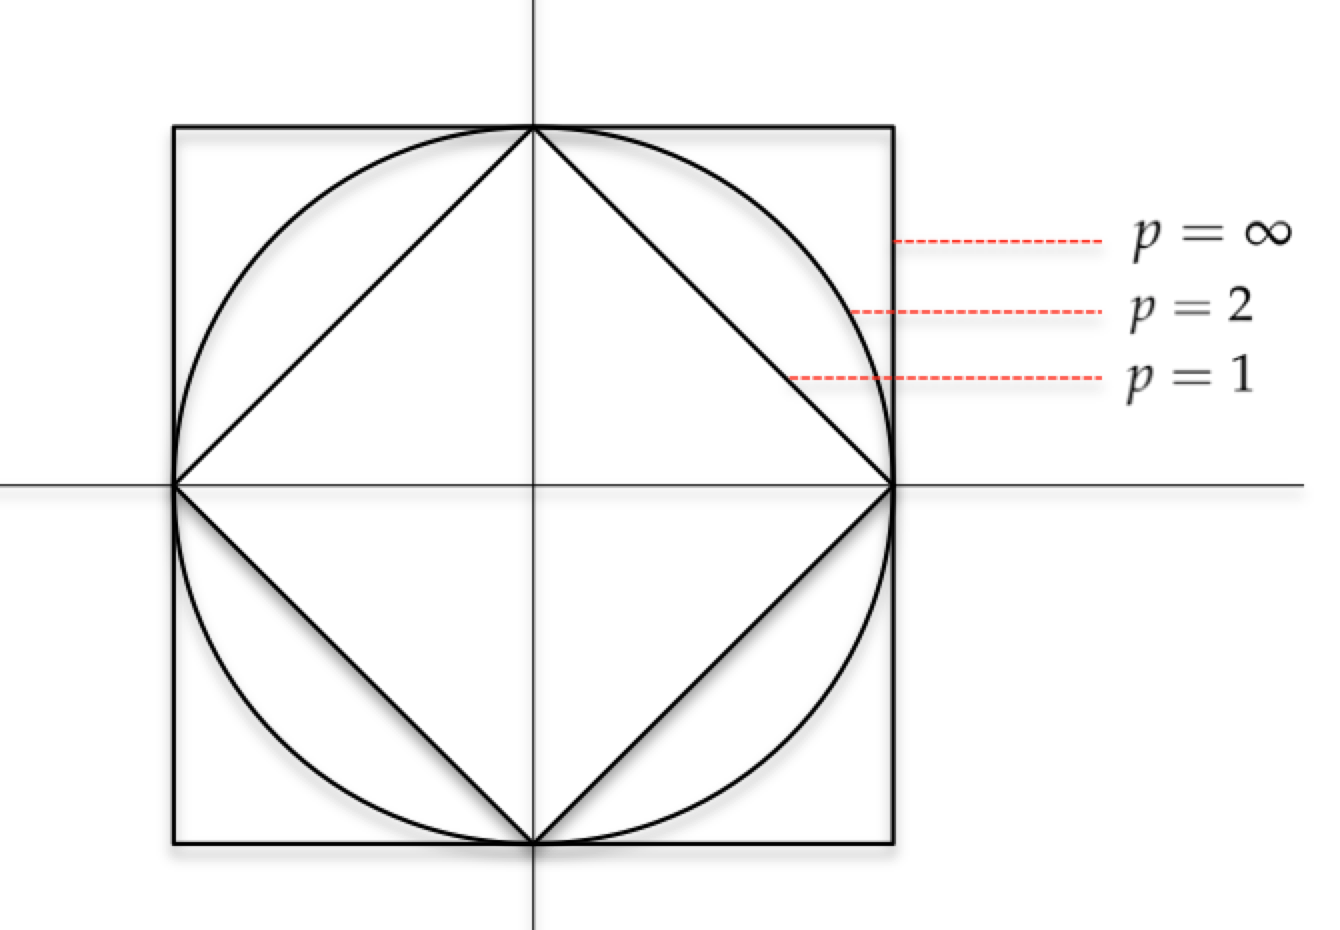
\includegraphics[scale=0.35]{figures/lpnorms}\caption{Norm Balls in $\mathbb{R}^2$}\end{center}\end{figure}

\noindent Figure 2 depicts the norm balls in $\mathbb{R}^2$ for the $\ell_p$ norms where $p=1,2,\infty$. Let's use our knowledge of norm balls to solve some maximization optimization problems.
\begin{example}
Given some non-zero vector $\mathbf{y}\in\mathbb{R}^n$, we want to find a vector $\mathbf{x}\in B_p(1)$ for $p=2,\infty$, such that the inner product of $\mathbf{x}$ and $\mathbf{y}$ is maximized. 

\noindent The first step here is to convert these words into the standard optimization form we had seen in the previous lecture. The optimization problem we are trying to solve here is
$$\max_{\|x\|_p\leqslant 1} \mathbf{x}^\top\mathbf{y}$$
Now, there are two cases for $p$:
\begin{itemize}
\item $p=2$. The optimization problem is $$\max_{\|x\|_2\leqslant 1} \mathbf{x}^\top\mathbf{y}$$ Recall that $$\mathbf{x}^\top\mathbf{y} = \|\mathbf{x}\|_2\|\mathbf{y}\|_2\cos\theta$$ The norm is as large as possible if $\mathbf{x}$ and $\mathbf{y}$ are collinear, i.e. they lie on the same line. This happens when $\theta=0^\circ$. Therefore, the solution to the optimization problem can be found using the optimizer $$\mathbf{x}_2^* = \frac{\mathbf{y}}{\|\mathbf{y}\|_2}$$ Therefore, the optimal solution is, $$\max_{\|x\|_2\leqslant 1} \mathbf{x}^\top\mathbf{y}=\|\mathbf{y}\|_2$$
\item $p=\infty$. The optimization problem is $$\max_{\|x\|_\infty\leqslant 1} \mathbf{x}^\top\mathbf{y}$$ From Figure 2 we can deduce that the inner product will be maximized at the corners of the square, i.e. $$\mathbf{x}_\infty^* = \sign(\mathbf{y})$$ Therefore, $$\max_{\|x\|_\infty\leqslant 1} \mathbf{x}^\top\mathbf{y} = |y_1| + |y_2| = \|\mathbf{y}\|_1$$ Notice that the optimal solution here is not unique. We get an optimal solution for the two cases where $\mathbf{x}_\infty^* = -1,1$.
\end{itemize}
\end{example}
\section{Hyperplanes and Halfspaces}
\begin{definition}
A hyperplane in $\mathbb{R}^n$ is a set of the form $$H = \left\{\mathbf{x}\in\mathbb{R}^n\,:\, \mathbf{a}^\top\mathbf{x} = b\right\}$$ where $\mathbf{a}\in \mathbb{R}^n$, $\mathbf{a}\neq 0$, and $b\in\mathbb{R}$ are given. 
\end{definition}
\noindent In general, a hyperplane in $\mathbb{R}^n$ is an $(n-1)$-dimensional subspace of $\mathbb{R}^n$. In one dimension, a hyperplane is a point. In two dimension, it is a line. In three dimensions, it is a plane. In more than three dimensions, we call it a hyperplane. We can also think of hyperplanes as the level sets of linear functions. 
\pagebreak
  \begin{figure}[h!]\begin{center}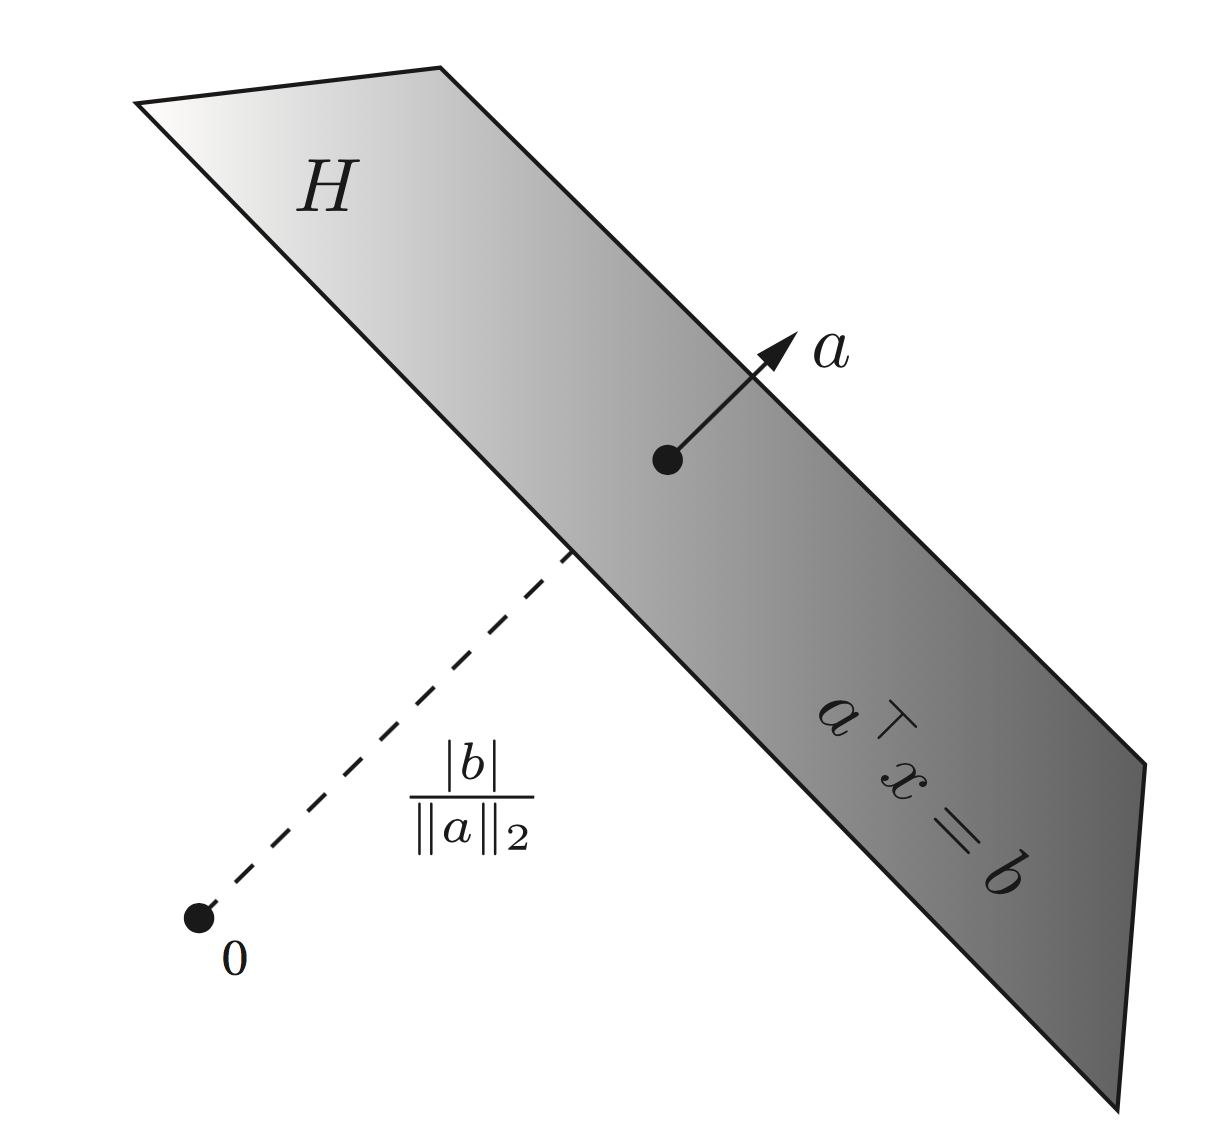
\includegraphics[scale=0.2]{figures/hyperplane}\caption{Example of a Hyperplane}\end{center}\end{figure}

\noindent In Figure 3 we see an example of a hyperplane.
\noindent Notice that when $b=0$, the hyperplane is simply the set of points that are orthogonal to $\mathbf{a}$. Now, we can think of a hyperplane as separating two regions in space: $$H_{-} = \left\{\mathbf{x}\,:\, \mathbf{a}^\top\mathbf{x}\leqslant b\right\},\quad H_{++} = \left\{\mathbf{x}\,:\, \mathbf{a}^\top\mathbf{x}> b\right\}$$ These two separated regions are called \textbf{halfspaces}. Notice that in $H_{-}$, it contains the value of $b$. This implies that $H_{-}$ is a closed halfspace while $H_{++}$ is an open halfspace.

  \begin{figure}[h!]\begin{center}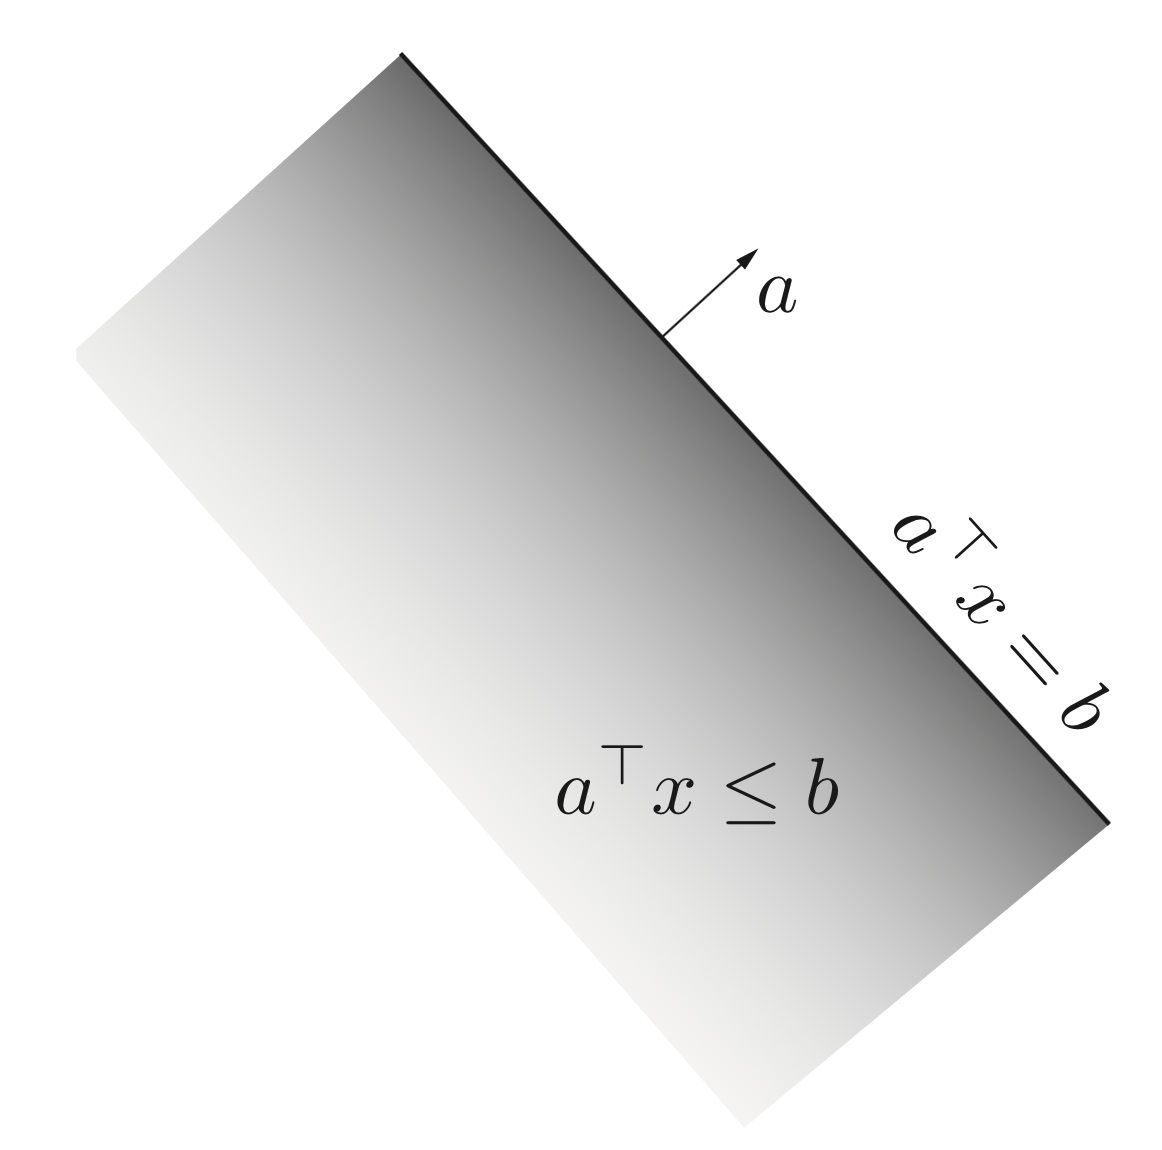
\includegraphics[scale=0.2]{figures/halfspace}\caption{Example of a Halfspace}\end{center}\end{figure}

\noindent In Figure 4 we see an example of the halfspace $H_{-}$. The halfspace $H_{-}$ is the region that lies in the direction opposite of vector $\mathbf{a}$, while the halfspace $H_{++}$ is the region lying above (in the direction of vector $\mathbf{a}$) the hyperplane. 

\section{Projections}
The idea of projection is central in optimization. It corresponds to the problem of finding a point on a given set that is closest to a given point. We can use different norms to define "closest". 
\begin{definition}
Given a vector $\mathbf{x}$ in an inner product space $V$, and a closed set $S\subseteq V$, the projection of $\mathbf{x}$ onto $S$, denoted as $\pi_S(\mathbf{x})$, is defined as the point in $S$ at minimal distance from $\mathbf{x}$: $$\pi_S(\mathbf{x}) = \arg\min_{\mathbf{y}\in S} \|\mathbf{y}-\mathbf{x}\|$$ where the norm used here is the norm induced by the inner product, that is $\|\mathbf{y}-\mathbf{x}\| = \sqrt{\langle \mathbf{y}-\mathbf{x}, \mathbf{y}-\mathbf{x}\rangle}$.
\end{definition}
\begin{theorem}
Projection Theorem. Let $\mathcal{X}$ be an inner product space. Let $\mathbf{x}$ be a given element in $\mathcal{X}$, and let $S$ be a subspace of $\mathcal{X}$. Then, there exists a unique vector $\mathbf{x}^*\in S$ which is the solution to the problem $$\min_{\mathbf{y}\in S} \|\mathbf{y}-\mathbf{x}\|$$ Moreover, a necessary and sufficient condition for $\mathbf{x}^*$ being the optimal solution for this problem is that $$\mathbf{x}^*\in S, \quad (\mathbf{x}-\mathbf{x}^*)\perp S$$
\end{theorem}

 \begin{figure}[h!]\begin{center}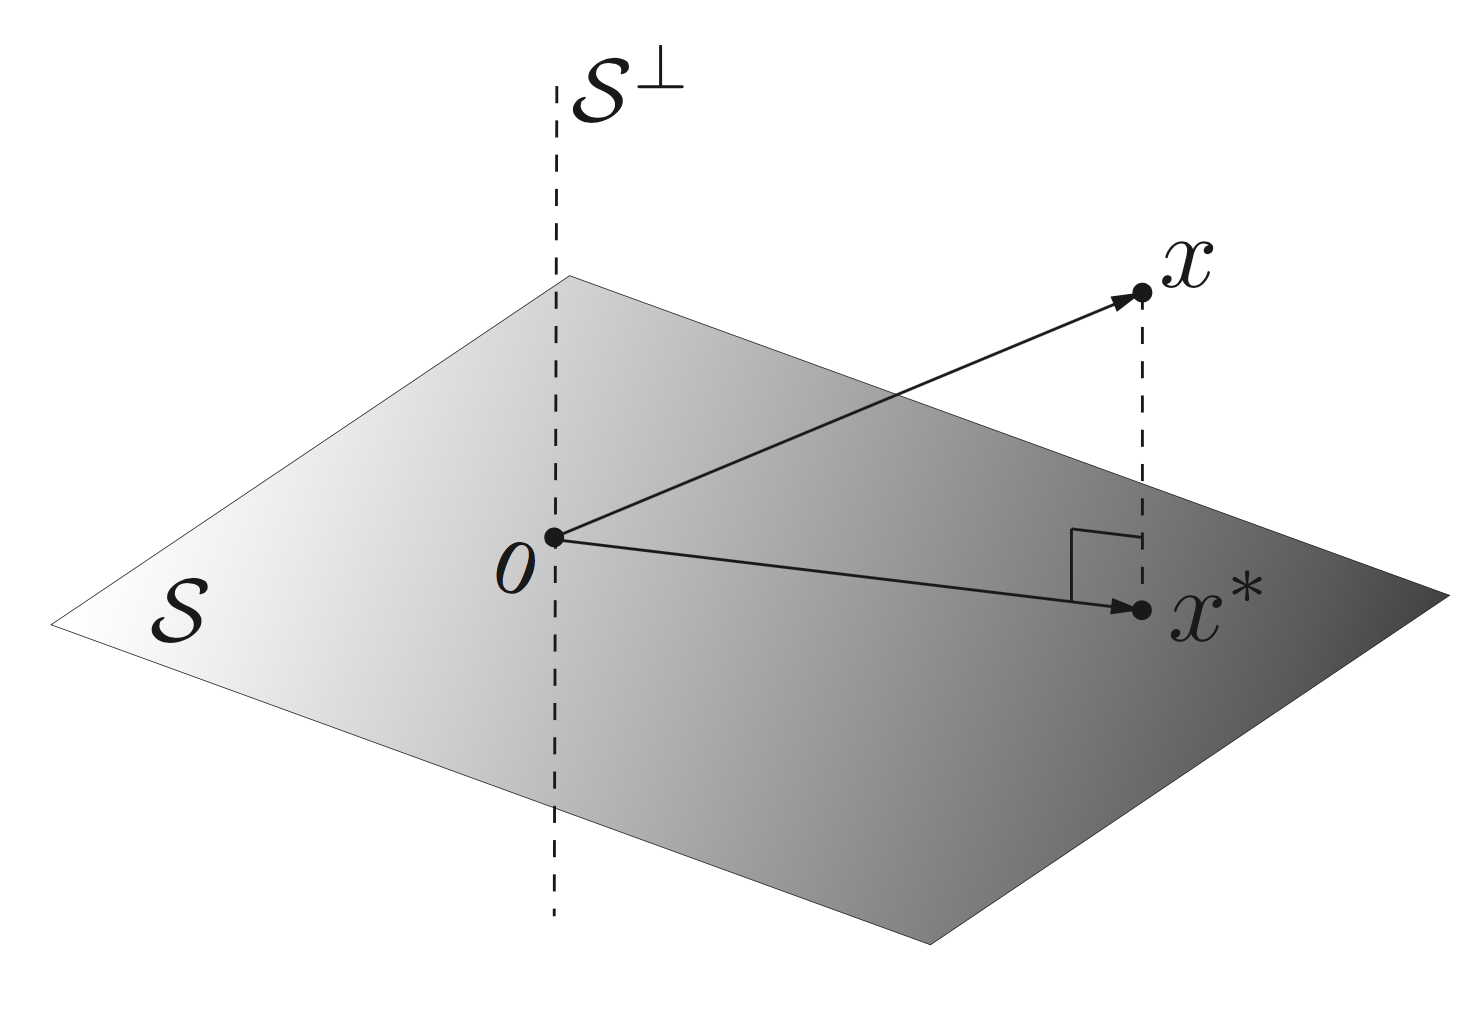
\includegraphics[scale=0.3]{figures/proj1}\caption{Projection Theorem Depiction}\end{center}\end{figure}

\noindent Notice in Figure 5 that $\mathbf{x}^*$ is the projection of $\mathbf{x}$ onto $S$. Additionally, $S^\perp$ is the orthogonal complement of $S$. By the Projection Theorem, this point is also the optimal solution to the minimization problem  $$\min_{\mathbf{y}\in S} \|\mathbf{y}-\mathbf{x}\|$$

\begin{corollary}
Projection on Affine Set. Let $\mathcal{X}$ be an inner product space, let $\mathbf{x}$ be a given element in $\mathcal{X}$, and let $\mathcal{A}=\mathbf{x}_0 + S$ be the affine set obtained by translating a given subspace $S$ by a given vector $\mathbf{x}_0$. Then, there exists a unique vector $\mathbf{x}^*\in\mathcal{A}$ which is the solution to the problem $$\min_{\mathbf{y}\in A} \|\mathbf{y}-\mathbf{x}\|$$ Moreover, a necessary and sufficient condition for $\mathbf{x}^*$ to be the optimal solution for this problem is that $$\mathbf{x}^*\in \mathcal{A},\quad (\mathbf{x}-\mathbf{x}^*)\perp S$$
\end{corollary}

\begin{figure}[h!]\begin{center}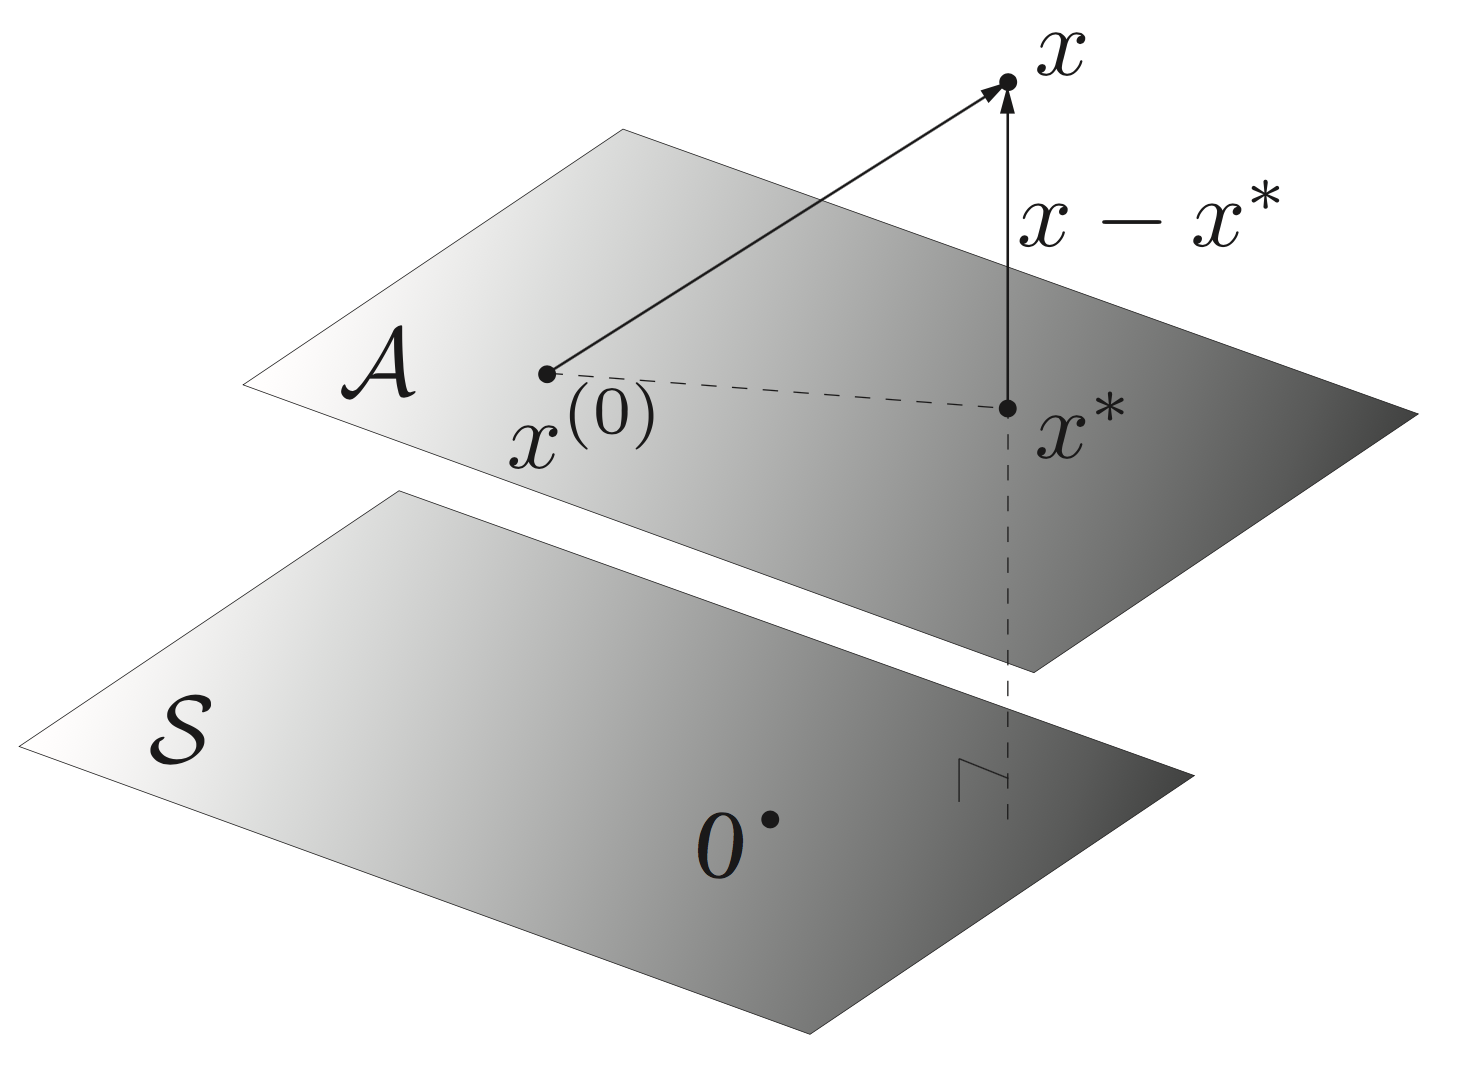
\includegraphics[scale=0.3]{figures/proj2}\caption{Projection on Affine Set}\end{center}\end{figure}

\noindent In Figure 6 we see a depiction of a projection on an affine set. Notice the similarities between Figure 5 and Figure 6. It almost seems that Figure 6 is a translation of Figure 5. And this is true, due to the definition of an affine set.

\subsection{Euclidean Projection of a Point onto a Line}
\begin{figure}[h!]\begin{center}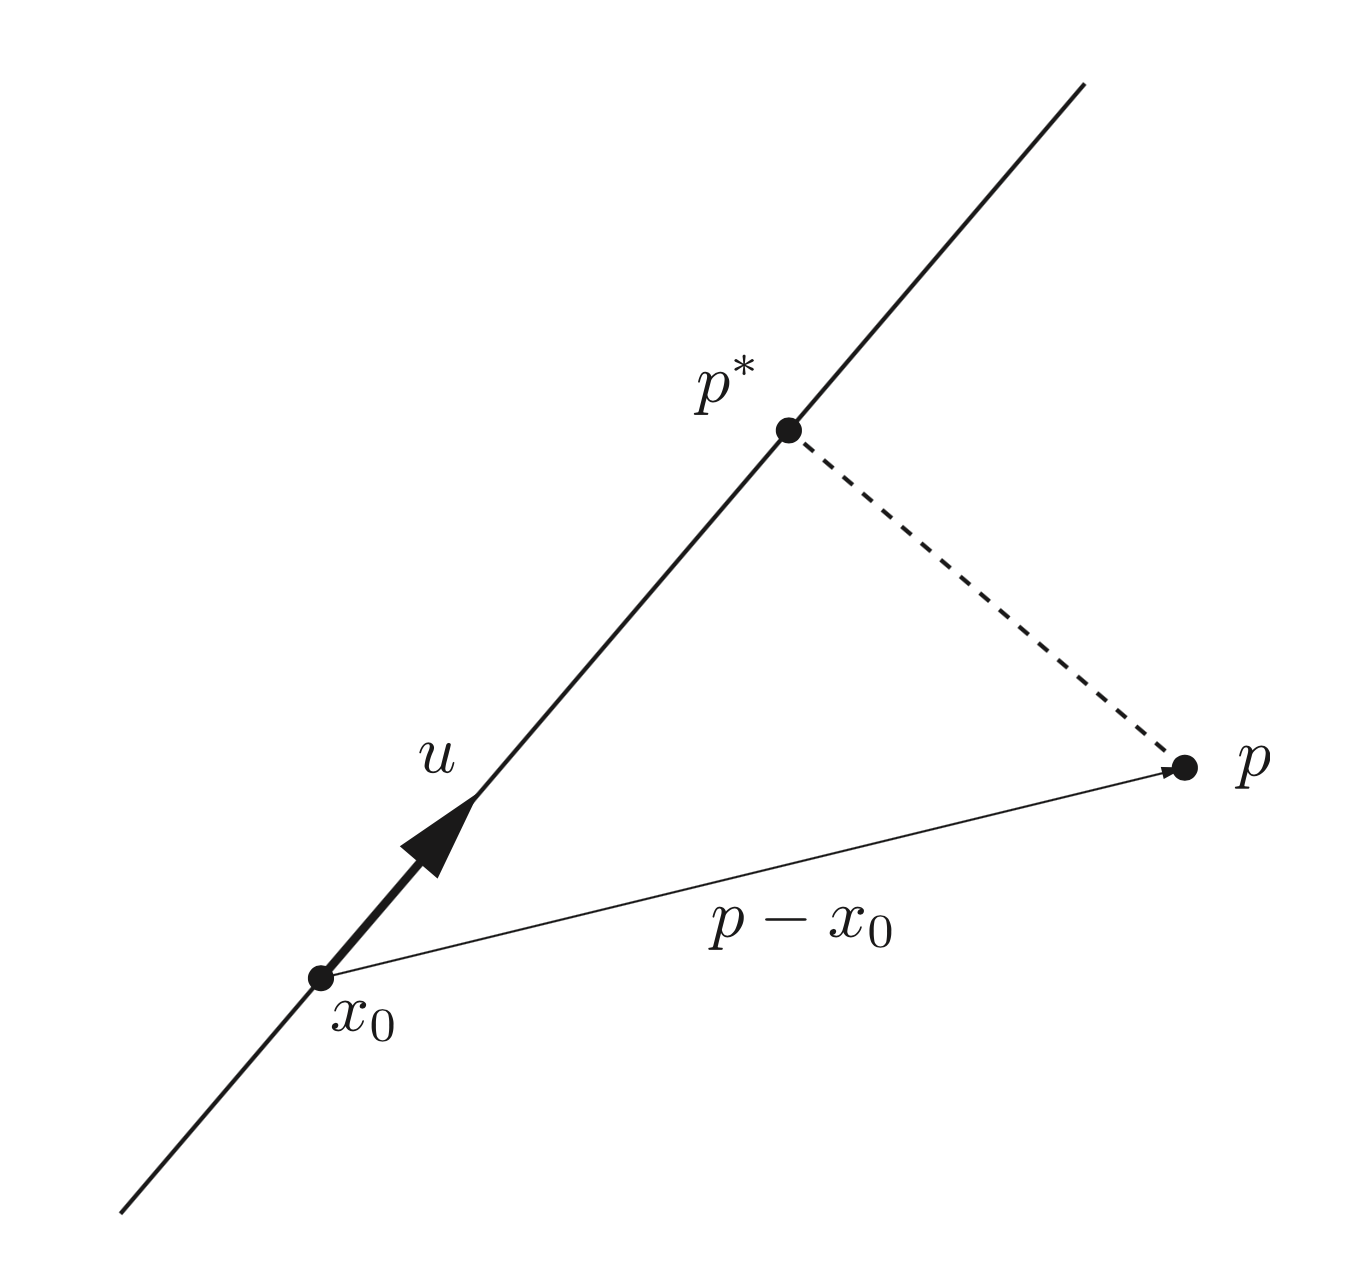
\includegraphics[scale=0.24]{figures/proj3}\caption{Euclidean Projection of a Point onto a Line}\end{center}\end{figure}

\noindent Let $\mathbf{p}\in\mathbb{R}^n$ be a given point. We want to compute the Euclidean projection $\mathbf{p}^*$ of $\mathbf{p}$ on to a line $L=\{\mathbf{x}_0 + \operatorname{span}(\mathbf{u})\}$, $\|\mathbf{u}\|_2=1$. In Figure 7 we see a depiction of the problem at hand. We want to find the point $\mathbf{p}^*$. We know from the Projection Theorem that $$\mathbf{p}^* = \arg\min_{\mathbf{x}\in L} \|\mathbf{x}-\mathbf{p}\|_2$$ Now, since any point $\mathbf{x}\in L$ can be written as $\mathbf{x} = \mathbf{x}_0 + \mathbf{v}$, for some $\mathbf{v}\in \operatorname{span}(\mathbf{u})$, the problem is equivalent to finding a value $\mathbf{v}^*$ for $\mathbf{v}$ such that $$\mathbf{v}^* = \arg\min_{\mathbf{v}\in \operatorname{span}(\mathbf{u})}\|\mathbf{v}-(\mathbf{p}-\mathbf{x}_0)\|_2$$ Let $\mathbf{z} = \mathbf{p} - \mathbf{x}_0$. Now, again from the Projection Theorem, we know that the solution must satisfy the orthogonality condition $(\mathbf{z} - \mathbf{v}^*)\perp \mathbf{u}$. Recall that $\mathbf{v}^* = \lambda^*\mathbf{u}$ and $\mathbf{u}^\top\mathbf{u} = \|\mathbf{u}\|_2^2 = 1$. Therefore, $$\mathbf{u}^\top\mathbf{z} - \mathbf{u}^\top\mathbf{v}^* = 0 \iff \mathbf{u}^\top\mathbf{z} - \lambda^* = 0\iff \lambda^* = \mathbf{u}^\top\mathbf{z} = \mathbf{u}^\top(\mathbf{p}-\mathbf{x}_0)$$ Thus, the optimal point $\mathbf{p}^*$ is given by $$\mathbf{p}^* = \mathbf{x}_0 + \mathbf{v}^* = \mathbf{x}_0 + \lambda^*\mathbf{u} = \mathbf{x}_0 + \mathbf{u}^\top(\mathbf{p}-\mathbf{x}_0)$$ and the squared distance from the point $\mathbf{p}$ to the line is $$\|\mathbf{p} - \mathbf{p}^*\|_2^2 = \|\mathbf{p}-\mathbf{x}_0\|_2^2 - {\lambda^*}^2 = \|\mathbf{p}-\mathbf{x}_0\|_2^2 - \left(\mathbf{u}^\top(\mathbf{p}-\mathbf{x}_0)\right)^2$$

\subsection{Euclidean Projection of a Point onto a Hyperplane}
We previously saw the case of euclidean projection of a point onto a line. Now, we will consider the case of euclidean projection of a point on any arbitrary hyperplane. Recall that a hyperplane is an affine set defined as $$H=\{\mathbf{z}\in\mathbb{R}^n\,:\, \mathbf{a}^\top\mathbf{z} = b$$ where $\mathbf{a}\neq\mathbf{0}$ is called a normal direction of the hyperplane, since for any two vectors $\mathbf{z}_1,\mathbf{z}_2\in H$, it holds that $(\mathbf{z}_1-\mathbf{z}_2)\perp \mathbf{a}$. Now, given a point $\mathbf{p}\in\mathbb{R}^n$, we want to determine the euclidean projection $\mathbf{p}^*$ of $\mathbf{p}$ onto $H$. By the Projection Theorem, we need $(\mathbf{p}-\mathbf{p}^*_2)\perp H$. Since $\mathbf{a}$ is orthogonal to $H$, this is equivalent to saying that $\mathbf{p}-\mathbf{p}^* = \alpha\mathbf{a}$, for some $\alpha\in\mathbb{R}$. 

\noindent Now, to find $\alpha$, consider that $\mathbf{p}^*\in H$. Therefore, $\mathbf{a}^\top\mathbf{p}^*=b$. Now, considering the optimality condition $$\mathbf{p}-\mathbf{p}^* = \alpha\mathbf{a}$$ and multiplying it by $\mathbf{a}^\top$ on the left, i.e. $\mathbf{a}^\top\mathbf{p}$ instead of $\mathbf{p}^\top\mathbf{a}$, we get $$\mathbf{a}^\top\mathbf{p} - \mathbf{a}^\top\mathbf{p}^* = \alpha\mathbf{a}^\top\mathbf{a}\implies \mathbf{a}^\top\mathbf{p} - b = \alpha\|\mathbf{a}\|_2^2$$ Therefore, $$\alpha = \frac{\mathbf{a}^\top\mathbf{p} - b}{\|\mathbf{a}\|_2^2}\implies \mathbf{p}^* = \mathbf{p} - \frac{\mathbf{a}^\top\mathbf{p} - b}{\|\mathbf{a}\|_2^2}\mathbf{a}$$ Now, to find the distance from point $\mathbf{p}$ to hyperplane $H$, we do $$\|\mathbf{p}-\mathbf{p}^*\|_2 = |\alpha|\cdot \|\mathbf{a}\|_2 = \frac{|\mathbf{a}^\top\mathbf{p} - b|}{\|\mathbf{a}\|_2}$$

\subsection{Projection on a Vector Span}
Now, we consider projection on a vector span. Suppose that we have a basis for a subspace $S\subseteq V$, that is 
$$S = \operatorname{span}(\mathbf{x}_1,\ldots,\mathbf{x}_d)$$ Given that $\mathbf{x}\in V$, by the Projection 
Theorem, the unique projection $\mathbf{x}^*$ of  $\mathbf{x}$ onto $S$ is characterized by $(\mathbf{x}-\mathbf{x}
^*)\perp S$. Since $\mathbf{x}^*\in S$, we can write $\mathbf{x}^*$ as some linear combination of the elements in 
the basis of $S$, i.e. $$\mathbf{x}^* = \sum_{i=1}^d\alpha_i\mathbf{x}_i$$ Then, $(\mathbf{x}-\mathbf{x}^*)\perp 
S\iff \langle \mathbf{x}-\mathbf{x}^*, \mathbf{x}_k\rangle = 0$, for $k=1,\ldots,d$: $$\sum_{i=1}^d \alpha_i\langle 
\mathbf{x}_k, \mathbf{x}_i\rangle = \langle \mathbf{x}_k,\mathbf{x}\rangle,\quad\text{for } k=1,\ldots,d$$ Notice that 
this is a system of linear equations. More specifically these are known as Gram equations. Solving this system of 
linear equations gives us the coefficients $\alpha$, which then gives us $\mathbf{x}^*$.

\subsection{Projection onto the Span of Orthonormal Vectors}
Now, if we have an orthonormal basis for a subspace $S = \operatorname{span}(S)$, then we can immediately obtain the projection $\mathbf{x}^*$ of $\mathbf{x}$ onto that subspace. This is because the Gram equations immediately give us the coefficients $$\alpha_k = \langle\mathbf{x}_k,\mathbf{x}\rangle, \quad k = 1,\ldots, d$$ Thus, e have that $$\mathbf{x}^* = \sum_{i=1}^d\langle\mathbf{x}_i,\mathbf{x}\rangle\mathbf{x}_i$$ Now, given a basis $S = \{\mathbf{x}_1,\ldots,\mathbf{x}_d\}$ for a subspace $S = \operatorname{span}(S)$, we can use the \href{https://en.wikipedia.org/wiki/Gram%E2%80%93Schmidt_process}{Gram-Schmidt process} or \href{https://en.wikipedia.org/wiki/QR_decomposition}{QR factorization} to construct the orthonormal basis for the same subspace.
\section{Functions and Maps}
The term \textbf{map} usually reserved for vector-valued functions. Maps are functions that return a vector of values. We denote a map $f$ as $$f\,:\,\mathbb{R}^n\to\mathbb{R}^m$$ $f$ is a map with input space $\mathbb{R}^n$, a $n$-dimensional vector, and output space $\mathbb{R}^m$, a $m$-dimensional vector. The components of the map $f$ are the scalar-valued functions $f_i$ where $i=1,\ldots,m$. 

\noindent Now, consider the function $f\,:\,\mathbb{R}^n\to \mathbb{R}$. The \textbf{graph} of $f$ is denoted as the set of the input-output pairs that $f$ can attain, i.e. $$\operatorname{graph} f = \left\{(\mathbf{x},f(\mathbf{x}))\in\mathbb{R}^{n+1}\,:\,\mathbf{x}\in\mathbb{R}^n\right\}$$ The \textbf{epigraph} of $f$ is denoted as the set of the input-output pairs that $f$ can achieve, as well as "anything above" it, i.e. $$\operatorname{epi} f = \left\{(\mathbf{x},t)\in\mathbb{R}^{n+1}\,:\,\mathbf{x}\in\mathbb{R}^n, t\geqslant f(\mathbf{x})\right\}$$ There is a similar notion of a \textbf{hypograph} which denotes the set of input-output pairs that $f$ can achieve, as well as "anything below".
 \begin{figure}[h!]\begin{center}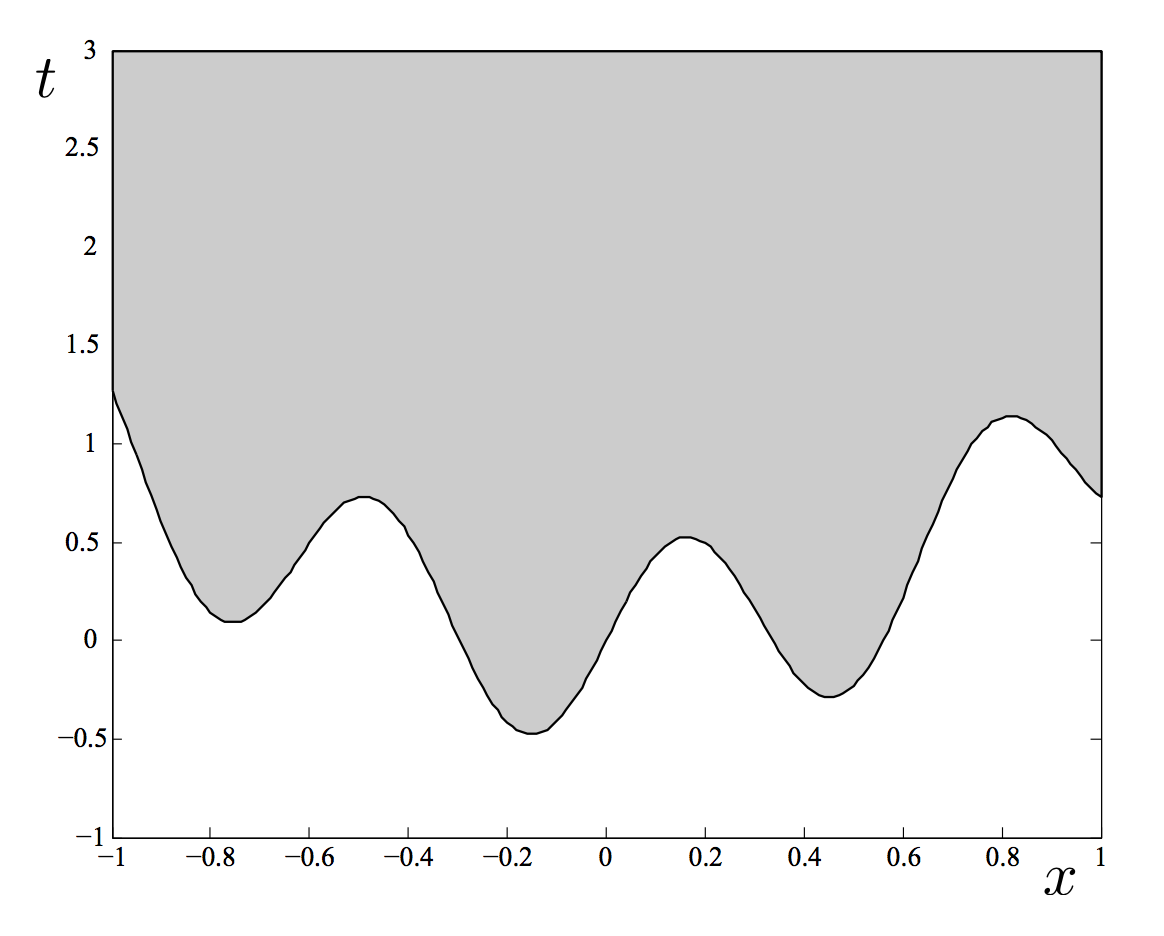
\includegraphics[scale=0.4]{figures/graph}\caption{Example of the Graph and Epigraph of a Function}\end{center}\end{figure}
 
 \noindent Figure 8 depicts the graph (black line) and epigraph (black line and shaded gray region) of some function $f$. 
 

\noindent Recall from last lecture that a level set (or contour line) is the set of points that achieve some value for the function $f$, i.e. for $t\in\mathbb{R}$, the $t$-level set of the function $f$ is defined as $$C_f(t) = \{\mathbf{x}\in\mathbb{R}^n\,:\,f(\mathbf{x})=t\}$$ Additionally, the $t$-sublevel set of $f$ is the set of points that achieve at most a certain value for $f$, i.e. $$L_f(t) = \{\mathbf{x}\in\mathbb{R}^n\,:\, f(\mathbf{x})\leqslant t\}$$

  \begin{figure}[h!]\begin{center}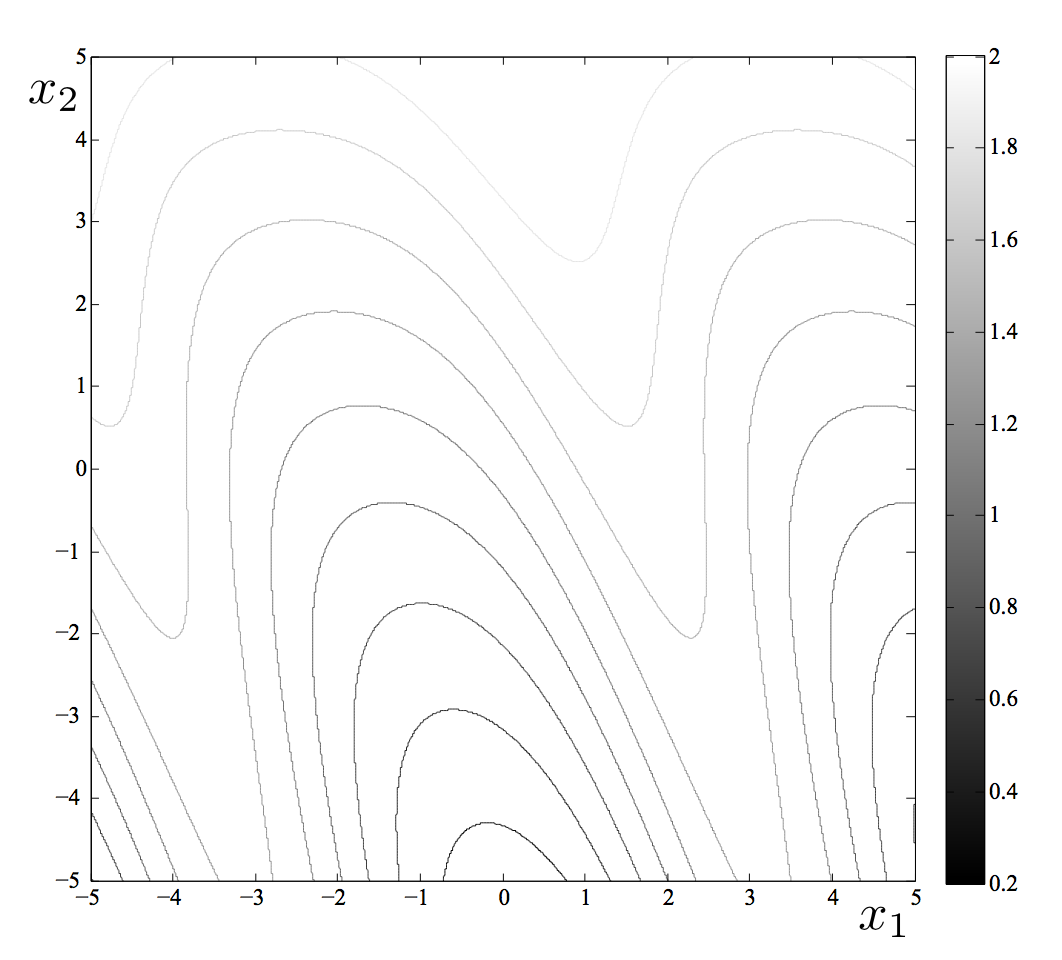
\includegraphics[scale=0.4]{figures/levelsets}\caption{Example of Level Sets}\end{center}\end{figure}
  
 \noindent Figure 9 depicts the level sets of a function.

\section{Linear and Affine Functions}
There are two types of functions that we will discuss here: linear functions and affine functions. Linear functions are functions that preserve scaling and addition of the input argument. More concretely,
\begin{definition}
A function $f\,:\,\mathbb{R}^n\to\mathbb{R}$ is \textbf{linear} if and only if $$\forall \mathbf{x}\in\mathbb{R}^n\,\,\text{and}\,\, c\in\mathbb{R}, f(c\mathbf{x}) = cf(\mathbf{x});$$ $$\forall\mathbf{x}_1,\mathbf{x}_2\in\mathbb{R}^n, f(\mathbf{x}_1+\mathbf{x}_2) = f(\mathbf{x}_1) + f(\mathbf{x}_2)$$
\end{definition}
\noindent In words, a linear function is simply a map between two vector spaces that preserves vector addition and scalar multiplication.

\begin{definition}
A function $f$ is \textbf{affine} if and only if the function $\tilde{f}(\mathbf{x}) = f(\mathbf{x})- f(\mathbf{0})$ is linear.
\end{definition}
\noindent Notice that we can rewrite $\tilde{f}(\mathbf{x}) = f(\mathbf{x}) - f(\mathbf{0})$ as $f(\mathbf{x}) = \tilde{f}(\mathbf{x}) + f(\mathbf{0})$, i.e. an affine function is the sum of a linear function and some constant. Therefore, the main difference between a linear function and an affine function is that a linear function fixes the origin, while an affine function doesn't. Moreover, an affine function is essentially some translated linear function. 
\begin{example}
Consider the following functions:
\begin{itemize}
\item The function $f_1(\mathbf{x}) = 3.2x_1+2x_2$ is a linear function.
\item The function $f_2(\mathbf{x}) = 3.2x_1+2x_2 + 0.15$ is an affine function.
\item The function $f_3(\mathbf{x}) = 2.1x_2^2 + 3.2x_1+2x_2$ is neither a linear function nor an affine function. If is a quadratic function.
\end{itemize}
\end{example}
\noindent Now, we can define both linear functions and affine functions in terms of an inner product.
\begin{definition}
A function $f\,:\, \mathbb{R}^n\to \mathbb{R}$ is affine if and only if it can be expressed as $$f(\mathbf{x}) = \mathbf{a}^\top\mathbf{x} + b$$ for $\mathbf{a}\in\mathbb{R}^n$ and $b\in\mathbb{R}$.
\end{definition}
\noindent Using this definition, we can conclude that a function is linear if and only if $b=0$.

\section{Affine Approximation of Nonlinear Functions}
We can approximate non-linear functions via an affine function. Recall Taylor's theorem:
\begin{theorem}
Taylor's Theorem. Suppose that $f\,:\,\mathbb{R}^n\to\mathbb{R}$ is continuously differentiable. Let $\mathbf{h}\in\mathbb{R}^n$. Then, there exists a $\lambda\in (0,1)$ such that $$f(\mathbf{x}+\mathbf{h}) = f(\mathbf{x}) + \nabla f(\mathbf{x}+ \lambda\mathbf{h})^\top\mathbf{h}$$ Now, if $f$ is twice continuously differentiable, then $$\nabla f(\mathbf{x}+\mathbf{h}) = \nabla f(\mathbf{x}) + \int_0^1 \nabla^2 f(\mathbf{x}+\lambda\mathbf{h})\mathbf{h}\,dt$$ and there exists a $\lambda\in (0,1)$ such that $$f(\mathbf{x}+\mathbf{h}) = f(\mathbf{x}) + \nabla f(\mathbf{x})^\top\mathbf{h} + \frac{1}{2!}\mathbf{h}^\top\nabla^2f(\mathbf{x}+\lambda \mathbf{h})\mathbf{h}$$
\end{theorem}

\noindent You may be familiar with another version of Taylor's theorem. This is a generalization of that theorem in multi-dimensions. Now, if $f\,:\,\mathbb{R}^n\to\mathbb{R}$ is some non-linear function, we can use Taylor's theorem to compute an affine function that can approximate $f$. Moreover, if $f$ is differentiable at a point $\mathbf{x}_0$, then from Taylor's theorem, for all points $\mathbf{x}$ in a neighborhood of $\mathbf{x}_0$, we have that $$f(\mathbf{x}) = f(\mathbf{x}_0) + \nabla f(\mathbf{x}_0)^\top(\mathbf{x}-\mathbf{x}_0) + \epsilon(\mathbf{x})$$ where $\epsilon(\mathbf{x})$ is some perturbation that goes to zero faster than first order, i.e. $$\lim_{\mathbf{x}\to\mathbf{x}_0} \frac{\epsilon(\mathbf{x})}{\|\mathbf{x}-\mathbf{x}_0\|_2} \to 0$$ Now, in practice, we typically use the first order expansion. For $\mathbf{x}$ sufficiently close to $\mathbf{x}_0$, we write that $$f(\mathbf{x})\approx f(\mathbf{x}_0) + \nabla f(\mathbf{x}_0)^\top(\mathbf{x}-\mathbf{x}_0)$$ We will understand this in more detail later when we discuss the Hessian matrix.

\section{Gradients}
\textbf{Gradients} generalize the concept of differentiation to scalar functions of multiple variables. The gradient of a function $f\,:\,\mathbb{R}^n\to\mathbb{R}$ at a point $\mathbf{x}$, given that $f$ is differentiable at the point $\mathbf{x}$, is denoted by $\nabla f(\mathbf{x})$. We denote $\nabla f(\mathbf{x})$ as a column vector of the first derivatives of $f$ with respect to each of it's variables. If $x_1,\ldots,x_n$ are each of these variables, then $$\nabla f(\mathbf{x}) = \begin{bmatrix} \frac{\partial f(\mathbf{x})}{\partial x_1} \\ \vdots \\ \frac{\partial f(\mathbf{x})}{\partial x_n}\end{bmatrix}$$ Notice that when $n=1$, the gradient is simply the derivative we are accustomed to seeing. One interesting property of affine functions is that if $f\,:\,\mathbb{R}^n\to\mathbb{R}$ is affine, i.e. $f(\mathbf{x}) = \mathbf{a}^\top\mathbf{x}+b$, then the gradient is $\nabla f(\mathbf{x}) = \mathbf{a}$. 
\begin{example}
We want to find the gradient of the distance function $\|\mathbf{x}-\mathbf{p}\|_2$. There are multiple ways to approach this. Let's let $f(\mathbf{x}) = \|x\|_2$. We can find the gradient of $f$ as follows: $$f(\mathbf{x}) = \|\mathbf{x}\|_2 = (\mathbf{x}^\top\mathbf{x})^{1/2} = \left(\sum_{k=1}^n x_k^2\right)^{1/2}$$ Now, for any variable $x_j$, $1\leqslant j\leqslant n$. Therefore, $$\frac{\partial f(\mathbf{x})}{\partial x_j} = \frac{1}{2}\left(\sum_{k=1}^n x_k^2\right)^{-1/2}\cdot 2 x_j = \left(\sum_{k=1}^n x_k^2\right)^{-1/2}\cdot x_j = \frac{x_j}{\|\mathbf{x}\|_2}$$ Hence $$\nabla f(\mathbf{x}) = \frac{\mathbf{x}}{\|\mathbf{x}\|_2}$$
Now, notice that the distance function is simply $f(\mathbf{x}-\mathbf{p})$. Therefore, from the chain rule, we get that $$\nabla f(\mathbf{x}-\mathbf{p}) = \frac{\mathbf{x}-\mathbf{y}}{\|\mathbf{x} - \mathbf{y}\|_2}$$
\end{example}
\noindent Now we know what the gradient is defined as, but what does it look geometrically? We can interpret the gradient of a function in the context of level sets.

 \begin{figure}[h!]\begin{center}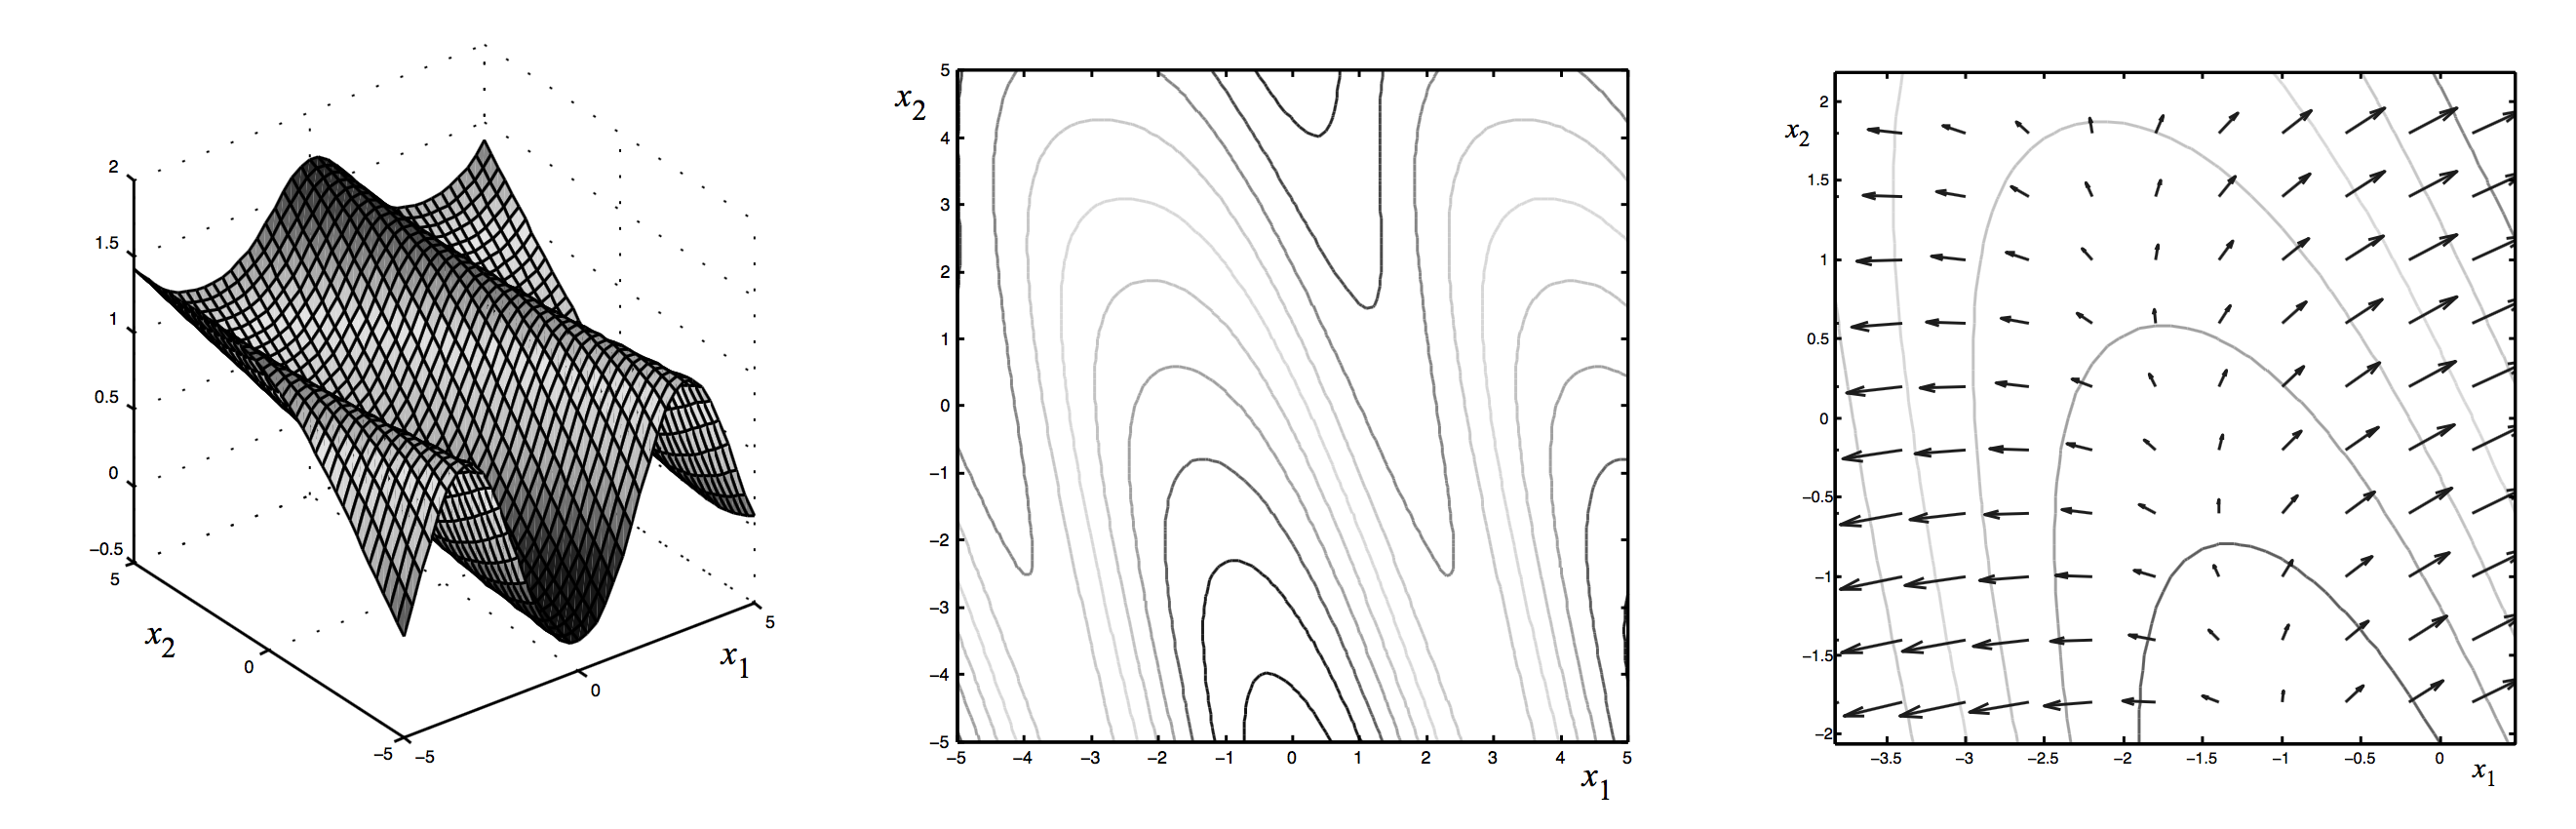
\includegraphics[scale=0.3]{figures/gradient1}\caption{Example for a Gradient}\end{center}\end{figure}
 
\noindent In Figure 10 we see 3 graphs. The first graph represents a function in $\mathbb{R}^3$. In the second graph, we see the level sets of the function. Now, the gradient of a function $f$ at a point $x_0$ is a vector $\nabla f(x_0)$ which is orthogonal to the contour line of $f$ at a level $\alpha = f(x_0)$, pointing outwards from $x_0$ at the $\alpha$-sublevel set. In the third graph we see this. Additionally, these gradient vectors tell us the direction of the steepest ascent, i.e. the direction in which we have the maximum rate of increase (think of stepping up a mountain). 

\nocite{*}
\bibliographystyle{alpha}
\bibliography{refs}

\end{document}
